% =====================================================================
% BMED365: Computational Imaging, Modeling and AI in Biomedicine
% Course Description and Topic List - Spring 2026
% =====================================================================
\documentclass[11pt,a4paper]{article}

% =====================================================================
% PACKAGES
% =====================================================================
\usepackage[utf8]{inputenc}
\usepackage[T1]{fontenc}
\usepackage[english]{babel}
\usepackage{graphicx}
\usepackage{booktabs}
\usepackage{longtable}
\usepackage{tabularx}
\usepackage{array}
\usepackage{multirow}
\usepackage{xcolor}
\usepackage{hyperref}
\usepackage{enumitem}
\usepackage{geometry}
\usepackage{fancyhdr}
\usepackage{titlesec}
\usepackage{tcolorbox}
\usepackage{amsmath}
\usepackage{amssymb}
\usepackage{natbib}
\usepackage{tikz}
\usetikzlibrary{shapes.geometric, arrows, positioning, mindmap}
\usepackage{multicol}

% =====================================================================
% LAYOUT AND FORMATTING
% =====================================================================
\geometry{margin=2.5cm}
\setlength{\parindent}{0pt}
\setlength{\parskip}{0.5em}

% Colors
\definecolor{uibblue}{RGB}{0, 61, 115}
\definecolor{uibred}{RGB}{175, 28, 44}
\definecolor{lightgray}{RGB}{245, 245, 245}
\definecolor{corecolor}{RGB}{0, 100, 0}
\definecolor{recommendedcolor}{RGB}{0, 0, 150}
\definecolor{optionalcolor}{RGB}{100, 100, 100}

% Hyperref
\hypersetup{
    colorlinks=true,
    linkcolor=uibblue,
    citecolor=uibblue,
    urlcolor=uibred
}

% Title formatting
\titleformat{\section}{\Large\bfseries\color{uibblue}}{\thesection}{1em}{}
\titleformat{\subsection}{\large\bfseries\color{uibblue!80}}{\thesubsection}{1em}{}
\titleformat{\subsubsection}{\normalsize\bfseries\color{uibblue!60}}{\thesubsubsection}{1em}{}

% Header/Footer
\pagestyle{fancy}
\fancyhf{}
\fancyhead[L]{\small\textcolor{gray}{BMED365 -- Spring 2026}}
\fancyhead[R]{\small\textcolor{gray}{Course Description and Topic List}}
\fancyfoot[C]{\thepage}
\renewcommand{\headrulewidth}{0.4pt}

% Box definitions
\newtcolorbox{infobox}[1][]{
    colback=lightgray,
    colframe=uibblue,
    title=#1,
    fonttitle=\bfseries,
    boxrule=0.5pt
}

\newtcolorbox{warningbox}[1][]{
    colback=uibred!5,
    colframe=uibred,
    title=#1,
    fonttitle=\bfseries,
    boxrule=0.5pt
}

% =====================================================================
% DOCUMENT START
% =====================================================================
\begin{document}

% =====================================================================
% TITLE PAGE
% =====================================================================
\begin{titlepage}
\centering
\vspace*{0.5cm}

{\Huge\bfseries\color{uibblue} BMED365}\\[0.3cm]
{\Large\bfseries Computational Imaging, Modeling and AI in Biomedicine}\\[0.6cm]

\rule{\textwidth}{1pt}\\[0.3cm]
{\LARGE Course Description and Topic List}\\[0.2cm]
{\large Spring 2026}\\[0.3cm]
\rule{\textwidth}{1pt}

\vspace{1cm}

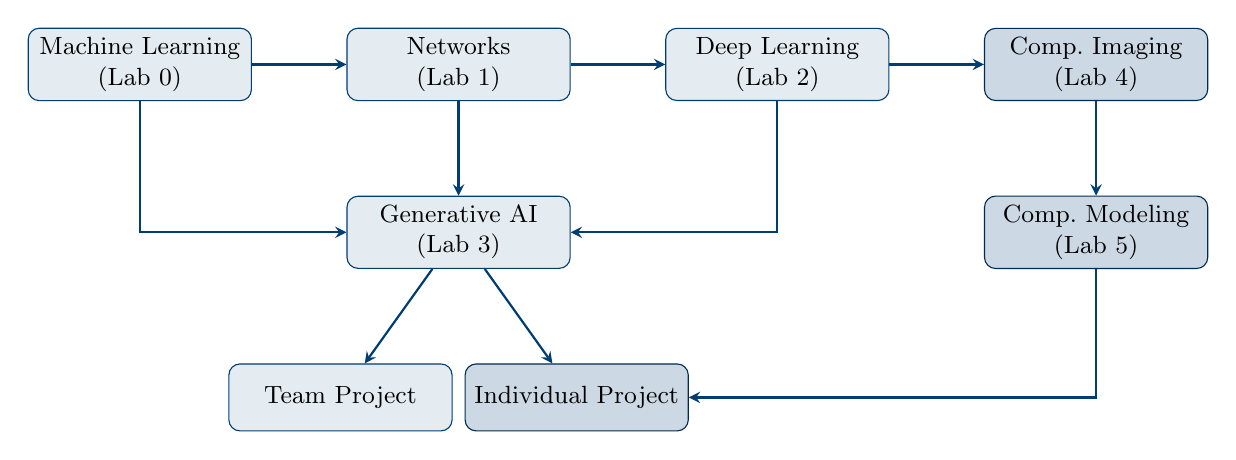
\begin{tikzpicture}[node distance=1.2cm, auto]
    % Styles
    \tikzstyle{block} = [rectangle, draw=uibblue, fill=uibblue!10, 
        text width=2.6cm, text centered, rounded corners, minimum height=0.85cm, font=\small]
    \tikzstyle{block2} = [rectangle, draw=uibblue!70!black, fill=uibblue!20, 
        text width=2.6cm, text centered, rounded corners, minimum height=0.85cm, font=\small]
    \tikzstyle{arrow} = [thick,->,>=stealth,uibblue]
    
    % Block 1 nodes (top row)
    \node [block] (ml) {Machine Learning\\(Lab 0)};
    \node [block, right=of ml] (net) {Networks\\(Lab 1)};
    \node [block, right=of net] (dl) {Deep Learning\\(Lab 2)};
    \node [block, below=of net] (genai) {Generative AI\\(Lab 3)};
    
    % Block 2 nodes (right column)
    \node [block2, right=of dl] (compimg) {Comp.\ Imaging\\(Lab 4)};
    \node [block2, below=of compimg] (compmod) {Comp.\ Modeling\\(Lab 5)};
    
    % Team/Individual projects
    \node [block, below=of genai, xshift=-1.5cm] (team) {Team Project};
    \node [block2, below=of genai, xshift=1.5cm] (indiv) {Individual Project};
    
    % Block 1 arrows
    \draw [arrow] (ml) -- (net);
    \draw [arrow] (net) -- (dl);
    \draw [arrow] (ml) |- (genai);
    \draw [arrow] (dl) |- (genai);
    \draw [arrow] (net) -- (genai);
    \draw [arrow] (genai) -- (team);
    
    % Block 2 arrows
    \draw [arrow] (dl) -- (compimg);
    \draw [arrow] (compimg) -- (compmod);
    \draw [arrow] (compmod) |- (indiv);
    \draw [arrow] (genai) -- (indiv);
\end{tikzpicture}

\vspace{1cm}

{\large
\textbf{Department of Biomedicine}\\
Faculty of Medicine\\
University of Bergen\\[0.5cm]
In collaboration with\\
Mohn Medical Imaging and Visualization Centre (MMIV)
}

\vspace{0.8cm}

\rule{0.6\textwidth}{0.4pt}

\vspace{0.5cm}

{\normalsize
\textbf{Course Responsible:} Arvid Lundervold\\[0.2cm]
\textbf{Course Material:} \url{https://github.com/arvidl/BMED365-2026}
}

\vfill
{\footnotesize December 2025}

\end{titlepage}

% =====================================================================
% TABLE OF CONTENTS
% =====================================================================
\tableofcontents
\newpage

% =====================================================================
% 1. INTRODUCTION AND MOTIVATION
% =====================================================================
\section{Introduction and Motivation}

\subsection{Why AI in Medicine?}

Artificial intelligence (AI) and machine learning are increasingly transforming healthcare and biomedical research \citep{topol2019high}. From image diagnostics and disease progression prediction to clinical decision support and drug development -- AI-based tools are becoming increasingly relevant for healthcare professionals and researchers.

\begin{infobox}[Core Questions of the Course]
\begin{itemize}[nosep]
    \item How do machine learning and deep learning work?
    \item How can AI be applied responsibly in medicine?
    \item What are the opportunities and limitations of current AI technology?
    \item What does \emph{precision medicine} mean in practice?
\end{itemize}
\end{infobox}

\subsection{The Course's Place in the Curriculum}

BMED365 is an elective course worth 10 ECTS credits offered to students with interest in AI in a health context. The course consists of two blocks: Block 1 (January) is shared with ELMED219, and Block 2 (February) includes additional labs on computational imaging and modeling.

\subsection{Learning Outcomes}

Upon completion of the course, the student should be able to:

\subsubsection*{Knowledge}
\begin{itemize}[nosep]
    \item Explain fundamental principles of machine learning, deep learning, and generative AI
    \item Describe network analysis and patient similarity networks (PSN)
    \item Account for ethical and regulatory aspects of medical AI
    \item Understand concepts such as \emph{explainable AI} (XAI) and \emph{trustworthy AI}
\end{itemize}

\subsubsection*{Skills}
\begin{itemize}[nosep]
    \item Apply Python and Jupyter Notebooks for simple ML analyses
    \item Use AI tools (ChatGPT, Gemini, Claude) as learning and work partners
    \item Construct and analyze patient similarity networks
    \item Write a research plan using LaTeX
\end{itemize}

\subsubsection*{General Competence}
\begin{itemize}[nosep]
    \item Assess opportunities and limitations of AI in clinical practice
    \item Reflect on ethical implications of AI technology
    \item Collaborate interdisciplinarily in project groups
    \item Communicate professionally about AI-related topics
\end{itemize}

% =====================================================================
% 2. COURSE STRUCTURE AND CONTENT
% =====================================================================
\section{Course Structure and Content}

\subsection{Overview of Activities}

The course is organized in two blocks. \textbf{Block 1} covers four laboratories (Labs 0--3), a quick start course, and a team project. \textbf{Block 2} covers computational imaging and modeling (Labs 4--5) and an individual project. Table~\ref{tab:activities} provides an overview.

\begin{table}[htbp]
\centering
\caption{Overview of course activities}
\label{tab:activities}
\begin{tabular}{@{}llp{5.5cm}c@{}}
\toprule
\textbf{Activity} & \textbf{Topic} & \textbf{Description} & \textbf{Hours} \\
\midrule
\multicolumn{4}{l}{\textit{Block 1}} \\
\midrule
Quick Start & AI-assisted Python & Intro to Python and AI tools & 4 \\
Lab 0 & Machine Learning & ML with scikit-learn and PyCaret & 6 \\
Lab 1 & Network Science & Graph theory and PSN with NetworkX & 6 \\
Lab 2 & Deep Learning & CNN and neural networks with PyTorch & 8 \\
Lab 3 & Generative AI \& LLM & Transformers, prompting, ethics & 6 \\
Team Project & Precision Medicine & Research plan for glioblastoma & 15 \\
\midrule
\multicolumn{4}{l}{\textit{Block 2}} \\
\midrule
Lab 4 & Comp.\ Imaging & MRI, imaging mass cytometry, segmentation & 6 \\
Lab 5 & Comp.\ Modeling & Physiological models, ODEs, simulations & 6 \\
Individual Project & Topic of Choice & Digital poster and speed presentation & 10 \\
\bottomrule
\end{tabular}
\end{table}

\subsection{Quick Start: AI-Assisted Python Programming}

The quick start course is designed for students without prior programming experience. It provides a practical introduction to:

\begin{itemize}[nosep]
    \item Google Colab and Jupyter Notebooks
    \item Python basics: variables, data types, lists, functions
    \item AI as a programming partner (Gemini/ChatGPT)
    \item Preview of Lab 0 (classification) and Lab 1 (networks)
\end{itemize}

\subsection{Lab 0: Machine Learning (ML)}

Lab 0 provides a practical introduction to machine learning with focus on classification and evaluation.

\begin{table}[htbp]
\centering
\caption{Notebooks in Lab 0}
\label{tab:lab0}
\begin{tabular}{@{}clp{7cm}@{}}
\toprule
\textbf{No.} & \textbf{Notebook} & \textbf{Content} \\
\midrule
01 & Simple examples & Features, labels, training, testing, decision trees \\
02 & Binary classification & Confusion matrix, ROC, precision, recall, F1-score \\
03 & PyCaret quick guide & AutoML for rapid prototyping \\
\bottomrule
\end{tabular}
\end{table}

\textbf{Learning Objectives:}
\begin{itemize}[nosep]
    \item Distinguish between supervised and unsupervised learning
    \item Use train/test split and cross-validation
    \item Interpret evaluation metrics (accuracy, precision, recall, AUC)
    \item Understand TRIPOD guidelines for medical ML
\end{itemize}

\subsection{Lab 1: Network Science and PSN}

Lab 1 introduces graph theory and the concept of \emph{patient similarity networks} (PSN) -- an approach for identifying patient subgroups based on similarity.

\begin{table}[htbp]
\centering
\caption{Notebooks in Lab 1}
\label{tab:lab1}
\begin{tabular}{@{}clp{6.5cm}@{}}
\toprule
\textbf{No.} & \textbf{Notebook} & \textbf{Content} \\
\midrule
00 & Introduction & Graph theory, adjacency matrices, centrality measures \\
01 & NetworkX tutorial & Create, manipulate, visualize graphs \\
02 & PSN with IRIS & Similarity calculation, community detection \\
03 & PSN with IBS data & Clinical application: brain and cognition \\
04 & PSN with IQ data & WAIS-IV and cognitive profiles \\
\bottomrule
\end{tabular}
\end{table}

\textbf{Learning Objectives:}
\begin{itemize}[nosep]
    \item Define graph, node, edge, and understand adjacency matrices
    \item Calculate centrality measures (degree, betweenness, eigenvector)
    \item Construct PSN from clinical data
    \item Apply the Louvain algorithm for community detection
\end{itemize}

\subsection{Lab 2: Deep Learning (DL)}

Lab 2 explores deep learning with focus on neural networks, CNN, and medical image analysis.

\begin{table}[htbp]
\centering
\caption{Notebooks in Lab 2 (prioritized)}
\label{tab:lab2}
\begin{tabular}{@{}cclp{5.5cm}@{}}
\toprule
\textbf{Part} & \textbf{Pri} & \textbf{Notebook} & \textbf{Content} \\
\midrule
A & 1 & CNN-intro & Conceptual intro to CNN \\
A & 1 & MNIST-MLP & Your first DL model \\
A & 1 & MNIST-CNN & CNN on handwritten digits \\
\midrule
B & 1 & NN-intro & Biological vs. artificial neurons \\
B & 1 & Learning in NN & Backpropagation, gradient descent \\
B & 1 & Heart disease & Classification from tabular data \\
B & 1 & ECG-arrhythmia & CNN on ECG signals \\
\midrule
C & 2 & CNN-architecture & Environment setup and architecture \\
C & 2 & CNN-training & Training and saving model \\
C & 2 & CNN-testing & Evaluation and Grad-CAM (XAI) \\
\midrule
D & 2 & MRI-dementia & MRI image analysis for dementia \\
\bottomrule
\end{tabular}
\end{table}

\textbf{Priority levels:} 1 = core, 2 = recommended, 3 = optional, 4 = advanced

\textbf{Learning Objectives:}
\begin{itemize}[nosep]
    \item Explain the structure of a neural network
    \item Understand backpropagation and gradient descent
    \item Build and train CNN with PyTorch
    \item Use Grad-CAM to interpret model decisions
\end{itemize}

\subsection{Lab 3: Generative AI and Large Language Models}

Lab 3 covers generative AI and large language models (LLM) with focus on medical applications, ethics, and explainability.

\begin{table}[htbp]
\centering
\caption{Notebooks in Lab 3}
\label{tab:lab3}
\begin{tabular}{@{}ccp{6cm}c@{}}
\toprule
\textbf{No.} & \textbf{Priority} & \textbf{Topic} & \textbf{Time} \\
\midrule
01 & \textcolor{corecolor}{Core} & Introduction to generative AI & 45 min \\
02 & \textcolor{corecolor}{Core} & Transformer architecture & 60 min \\
03 & \textcolor{corecolor}{Core} & LLM fundamentals (tokens, temp.) & 45 min \\
04 & \textcolor{corecolor}{Core} & Prompt engineering & 90 min \\
\midrule
05 & \textcolor{recommendedcolor}{Important} & Explainable AI (XAI) & 60 min \\
06 & \textcolor{recommendedcolor}{Important} & AI ethics in medicine & 60 min \\
\midrule
07 & \textcolor{optionalcolor}{Optional} & Trustworthy AI & 60 min \\
08 & \textcolor{optionalcolor}{Optional} & Neurosymbolic AI + Agentic AI & 90 min \\
09 & \textcolor{optionalcolor}{Optional} & ChatGPT/Claude API & 60 min \\
\bottomrule
\end{tabular}
\end{table}

\textbf{Note:} Notebook 08 (Neurosymbolic AI) contains a comprehensive \textbf{case study on brain tumors (glioma)} that demonstrates:
\begin{itemize}[nosep]
    \item Neurosymbolic classification based on WHO 2021 CNS classification
    \item Integration of MRI analysis (neural) with knowledge graphs (symbolic)
    \item Agentic AI orchestrating clinical workflow
\end{itemize}

\textbf{Learning Objectives:}
\begin{itemize}[nosep]
    \item Explain self-attention and transformer architecture
    \item Understand the difference between \emph{prompt engineering} and \emph{context engineering}
    \item Apply prompt engineering techniques (zero-shot, few-shot, CoT)
    \item Apply model-specific prompting techniques for GPT-5.2, Claude Opus 4.5, and Gemini 3
    \item Evaluate XAI methods such as SHAP and LIME
    \item Discuss AI ethics, bias, and EU AI Act
    \item Understand neurosymbolic integration of neural and symbolic methods
    \item Describe agentic AI and its role in clinical decision support
\end{itemize}

\subsection{Team Project: Precision Medicine for Glioblastoma}

The team project is a central part of the course where students in interdisciplinary groups develop a research plan (grant proposal sketch) for a hypothetical project on AI and imaging for brain tumors.

\begin{warningbox}[Important about the team project]
The task is to \textbf{write a research plan} -- not to actually implement the project with coding or data analysis.
\end{warningbox}

\textbf{Focus Areas:}
\begin{enumerate}[nosep]
    \item Imaging technologies and modalities (MRI, PET)
    \item Image-derived biomarkers for glioblastoma
    \item Machine learning techniques (segmentation, classification)
    \item Data management plan and ethical considerations
\end{enumerate}

\begin{infobox}[Relevant Background: The Glioma Case Study]
Notebook 08 in Lab 3 contains a comprehensive neurosymbolic AI case study for glioma classification based on WHO 2021 CNS classification. This demonstrates:
\begin{itemize}[nosep]
    \item Integration of MRI segmentation (BraTS) with molecular markers (IDH, MGMT, 1p/19q)
    \item Knowledge graphs for treatment recommendations
    \item Agentic AI for orchestrating clinical workflow
\end{itemize}
Students can use this as inspiration for the team project.
\end{infobox}

\textbf{Report Structure:}
\begin{itemize}[nosep]
    \item Research plan: 3--5 pages (background, objectives, methods, evaluation)
    \item Data management plan and ethics: 1.5--2.5 pages
    \item Written in English
    \item LaTeX template available on Overleaf
\end{itemize}

\subsection{Lab 4: Computational Imaging}

Lab 4 introduces computational imaging with focus on medical imaging modalities, image processing, and AI-based analysis.

\begin{table}[htbp]
\centering
\caption{Notebooks in Lab 4}
\label{tab:lab4}
\begin{tabular}{@{}clp{7cm}@{}}
\toprule
\textbf{No.} & \textbf{Notebook} & \textbf{Content} \\
\midrule
00 & Test installation & Verify environment and dependencies \\
01 & Imaging intro & Basic concepts in digital imaging \\
02 & MRI intro & Introduction to Magnetic Resonance Imaging \\
03 & IMC intro & Introduction to Imaging Mass Cytometry \\
\bottomrule
\end{tabular}
\end{table}

\textbf{Learning Objectives:}
\begin{itemize}[nosep]
    \item Understand fundamental concepts in computational imaging
    \item Explain basic principles of MRI and common sequences
    \item Describe imaging mass cytometry and its applications
    \item Apply image segmentation techniques
    \item Understand the role of AI in medical image analysis
\end{itemize}

\subsection{Lab 5: Computational Modeling}

Lab 5 explores computational modeling in biomedicine, including physiological models described by ordinary differential equations (ODEs).

\begin{table}[htbp]
\centering
\caption{Notebooks in Lab 5}
\label{tab:lab5}
\begin{tabular}{@{}clp{6.5cm}@{}}
\toprule
\textbf{No.} & \textbf{Notebook} & \textbf{Content} \\
\midrule
00 & Test LLM & Local LLM installation (DeepSeek-R1) \\
01 & Action potentials & Hodgkin-Huxley model of neuronal firing \\
02 & Tumor growth & Tumor growth and angiogenesis modeling \\
03 & Cardiovascular flow & Blood flow, ECG, and pressure waveforms \\
04 & Muscle force & Muscle force generation models \\
05 & Cell signaling & Cell signaling and gene regulatory networks \\
06 & Kidney filtration & LLM-assisted model generation \\
\bottomrule
\end{tabular}
\end{table}

\textbf{Learning Objectives:}
\begin{itemize}[nosep]
    \item Understand the role of mathematical models in biomedicine
    \item Describe and simulate the Hodgkin-Huxley model
    \item Model tumor growth dynamics
    \item Simulate cardiovascular flow and waveforms
    \item Use AI/LLM to assist in model development
\end{itemize}

\subsection{Individual Project: Digital Poster and Speed Presentation}

The individual project is completed between Block 1 and Block 2. Students work independently on a topic of their choice within the course scope.

\textbf{Deliverables:}
\begin{enumerate}[nosep]
    \item \textbf{Digital poster:} Submitted through Mitt UiB
    \item \textbf{Speed presentation:} 7-minute presentation + 3-minute discussion
\end{enumerate}

\textbf{Topic Selection:}
\begin{itemize}[nosep]
    \item Choose a topic covering computational imaging, modeling, or AI
    \item Can be based on own research, a scientific article, or a methods review
    \item Faculty guidance available for topic selection
\end{itemize}

\textbf{Assessment Criteria:}
\begin{itemize}[nosep]
    \item Scientific rigor and vocabulary
    \item Balanced content (text, tables, figures)
    \item Clear structure (introduction, methods, results, discussion, conclusions)
    \item Engagement and time management
\end{itemize}

% =====================================================================
% 3. DETAILED TOPIC LIST
% =====================================================================
\section{Detailed Topic List}

This section provides a comprehensive topic list organized by theme. Topics are marked with priority: \textbf{C} = core (mandatory), \textbf{I} = important (recommended), \textbf{S} = supplementary (optional).

\subsection{Machine Learning -- Fundamental Concepts}

\begin{longtable}{@{}clp{9cm}@{}}
\toprule
\textbf{Pri} & \textbf{No.} & \textbf{Topic} \\
\midrule
\endfirsthead
\multicolumn{3}{c}{\textit{Continued from previous page}} \\
\toprule
\textbf{Pri} & \textbf{No.} & \textbf{Topic} \\
\midrule
\endhead
\midrule
\multicolumn{3}{r}{\textit{Continues on next page}} \\
\endfoot
\bottomrule
\endlastfoot
C & M01 & Define \emph{machine learning} and distinguish from traditional programming \\
C & M02 & Explain the difference between \emph{supervised} and \emph{unsupervised} learning \\
C & M03 & Describe the concepts of \emph{features} (input) and \emph{labels} (output) \\
C & M04 & Explain why we split data into \emph{training} and \emph{test sets} \\
C & M05 & Define \emph{overfitting} and \emph{underfitting} \\
C & M06 & Understand \emph{bias-variance trade-off} \\
I & M07 & Describe k-fold \emph{cross-validation} and its advantages \\
I & M08 & Explain what a \emph{baseline model} is and why it is important \\
C & M09 & Distinguish between \emph{classification} and \emph{regression} \\
I & M10 & Know simple models: decision tree, k-NN, logistic regression \\
\end{longtable}

\subsection{Evaluation of ML Models}

\begin{longtable}{@{}clp{9cm}@{}}
\toprule
\textbf{Pri} & \textbf{No.} & \textbf{Topic} \\
\midrule
\endfirsthead
\midrule
\endhead
\midrule
\endfoot
\bottomrule
\endlastfoot
C & E01 & Interpret a \emph{confusion matrix} \\
C & E02 & Define TP, TN, FP, FN in medical context \\
C & E03 & Calculate and interpret \emph{accuracy} \\
C & E04 & Calculate and interpret \emph{precision} (PPV) \\
C & E05 & Calculate and interpret \emph{recall/sensitivity} \\
C & E06 & Calculate and interpret \emph{specificity} \\
I & E07 & Calculate and interpret \emph{F1-score} \\
C & E08 & Understand ROC curve and AUC as measures of model quality \\
I & E09 & Explain when accuracy is insufficient (imbalanced datasets) \\
I & E10 & Know TRIPOD guidelines for reporting \\
\end{longtable}

\subsection{Graph Theory and Network Science}

\begin{longtable}{@{}clp{9cm}@{}}
\toprule
\textbf{Pri} & \textbf{No.} & \textbf{Topic} \\
\midrule
\endfirsthead
\midrule
\endhead
\midrule
\endfoot
\bottomrule
\endlastfoot
C & N01 & Define what a \emph{graph} is (nodes and edges) \\
C & N02 & Distinguish between \emph{directed} and \emph{undirected} graphs \\
C & N03 & Distinguish between \emph{weighted} and \emph{unweighted} graphs \\
C & N04 & Represent a graph as an \emph{adjacency matrix} \\
C & N05 & Calculate \emph{degree centrality} and interpret the result \\
I & N06 & Calculate \emph{betweenness centrality} and interpret the result \\
I & N07 & Calculate \emph{eigenvector centrality} and interpret the result \\
I & N08 & Explain \emph{clustering coefficient} \\
I & N09 & Describe \emph{community detection} and the Louvain algorithm \\
C & N10 & Know the NetworkX library for Python \\
\end{longtable}

\subsection{Patient Similarity Networks (PSN)}

\begin{longtable}{@{}clp{9cm}@{}}
\toprule
\textbf{Pri} & \textbf{No.} & \textbf{Topic} \\
\midrule
\endfirsthead
\midrule
\endhead
\midrule
\endfoot
\bottomrule
\endlastfoot
C & P01 & Explain the concept of \emph{patient similarity networks} (PSN) \\
C & P02 & Describe how PSN can support \emph{precision medicine} \\
C & P03 & Calculate similarity between patients (Euclidean, Manhattan, Gower) \\
I & P04 & Construct a PSN from a patient-feature matrix \\
I & P05 & Choose threshold value for edge creation in PSN \\
I & P06 & Identify patient subgroups via community detection \\
S & P07 & Discuss advantages and limitations of the PSN approach \\
S & P08 & Know about multimodal PSN (integration of different data types) \\
\end{longtable}

\subsection{Neural Networks and Deep Learning}

\begin{longtable}{@{}clp{9cm}@{}}
\toprule
\textbf{Pri} & \textbf{No.} & \textbf{Topic} \\
\midrule
\endfirsthead
\midrule
\endhead
\midrule
\endfoot
\bottomrule
\endlastfoot
C & D01 & Compare biological and artificial neurons \\
C & D02 & Describe the structure of a \emph{multilayer perceptron} (MLP) \\
C & D03 & Explain what an \emph{activation function} is (ReLU, sigmoid) \\
C & D04 & Understand the concept of \emph{forward propagation} \\
C & D05 & Explain \emph{backpropagation} at a conceptual level \\
C & D06 & Understand \emph{gradient descent} and learning rate \\
I & D07 & Know about \emph{loss functions} (cross-entropy, MSE) \\
C & D08 & Describe a \emph{convolutional neural network} (CNN) \\
C & D09 & Explain what a \emph{convolution filter} does \\
C & D10 & Describe \emph{pooling layers} and their function \\
I & D11 & Know about \emph{batch normalization} and \emph{dropout} \\
I & D12 & Understand the concept of \emph{transfer learning} \\
S & D13 & Know about advanced architectures (ResNet, ViT) \\
\end{longtable}

\subsection{Generative AI and Large Language Models}

\begin{longtable}{@{}clp{9cm}@{}}
\toprule
\textbf{Pri} & \textbf{No.} & \textbf{Topic} \\
\midrule
\endfirsthead
\midrule
\endhead
\midrule
\endfoot
\bottomrule
\endlastfoot
C & G01 & Define \emph{generative AI} and distinguish from discriminative AI \\
C & G02 & Explain the \emph{self-attention} mechanism at a conceptual level \\
C & G03 & Describe the transformer architecture (encoder-decoder) \\
C & G04 & Explain what \emph{tokens} are and how tokenization works \\
C & G05 & Understand the concept of \emph{context window} \\
C & G06 & Explain what \emph{temperature} means in text generation \\
C & G07 & Apply \emph{zero-shot} prompting \\
C & G08 & Apply \emph{few-shot} prompting \\
I & G09 & Apply \emph{Chain-of-Thought} (CoT) prompting \\
I & G10 & Describe best practices for \emph{system prompts} \\
C & G11 & Define \emph{hallucination} and its implications \\
I & G12 & Know about GPT-5.2, Claude Opus 4.5, Gemini 3 and their strengths \\
S & G13 & Explain the concept of \emph{foundation model} \\
S & G14 & Describe RAG (Retrieval-Augmented Generation) \\
I & G15 & Understand the difference between \emph{prompt engineering} and \emph{context engineering} \\
I & G16 & Describe components of context engineering (system prompt, RAG, tools, conversation history) \\
I & G17 & Apply model-specific prompting techniques for GPT-5.2, Claude, and Gemini \\
I & G18 & Handle uncertainty and hallucination risk in medical prompts \\
S & G19 & Use structured extraction from medical documents (JSON schema) \\
S & G20 & Compare model strengths for different medical tasks \\
\end{longtable}

\subsection{Explainable AI (XAI)}

\begin{longtable}{@{}clp{9cm}@{}}
\toprule
\textbf{Pri} & \textbf{No.} & \textbf{Topic} \\
\midrule
\endfirsthead
\midrule
\endhead
\midrule
\endfoot
\bottomrule
\endlastfoot
C & X01 & Explain why explainability is important in medical AI \\
C & X02 & Distinguish between \emph{global} and \emph{local} explainability \\
I & X03 & Distinguish between \emph{ante-hoc} and \emph{post-hoc} explainability \\
I & X04 & Describe SHAP (SHapley Additive exPlanations) \\
I & X05 & Describe LIME (Local Interpretable Model-agnostic Explanations) \\
I & X06 & Explain Grad-CAM for CNN visualization \\
I & X07 & Discuss limitations of XAI methods \\
S & X08 & Know about attention visualization in LLM \\
\end{longtable}

\subsection{Trustworthy AI and Robustness}

\begin{longtable}{@{}clp{9cm}@{}}
\toprule
\textbf{Pri} & \textbf{No.} & \textbf{Topic} \\
\midrule
\endfirsthead
\midrule
\endhead
\midrule
\endfoot
\bottomrule
\endlastfoot
C & T01 & Define \emph{trustworthy AI} according to EU guidelines \\
I & T02 & Explain the concept of \emph{robustness} in ML \\
I & T03 & Describe \emph{distributional shift} and its consequences \\
I & T04 & Explain the difference between epistemic and aleatoric uncertainty \\
I & T05 & Describe \emph{human-in-the-loop} (HITL) systems \\
I & T06 & Discuss the importance of continuous monitoring \\
S & T07 & Know about adversarial attacks \\
\end{longtable}

\subsection{AI Ethics and Regulation}

\begin{longtable}{@{}clp{9cm}@{}}
\toprule
\textbf{Pri} & \textbf{No.} & \textbf{Topic} \\
\midrule
\endfirsthead
\midrule
\endhead
\midrule
\endfoot
\bottomrule
\endlastfoot
C & A01 & Discuss the four bioethical principles in AI context \\
C & A02 & Identify types of bias in medical AI systems \\
C & A03 & Explain privacy concerns when using LLM \\
C & A04 & Describe main features of EU AI Act \\
I & A05 & Explain risk classification in EU AI Act \\
I & A06 & Discuss requirements for high-risk AI in healthcare \\
C & A07 & Reflect on responsibility distribution when AI fails \\
I & A08 & Know about GDPR-relevant aspects of AI \\
S & A09 & Discuss algorithmic fairness \\
\end{longtable}

\subsection{Neurosymbolic AI and Agentic AI}

\begin{longtable}{@{}clp{9cm}@{}}
\toprule
\textbf{Pri} & \textbf{No.} & \textbf{Topic} \\
\midrule
\endfirsthead
\midrule
\endhead
\midrule
\endfoot
\bottomrule
\endlastfoot
S & S01 & Contrast symbolic and connectionist AI \\
S & S02 & Explain the concept of \emph{neurosymbolic integration} \\
S & S03 & Describe what a \emph{knowledge graph} is \\
S & S04 & Know about medical ontologies (SNOMED CT, ICD, WHO CNS classification) \\
S & S05 & Discuss potential advantages of neurosymbolic AI in medicine \\
S & S06 & Describe how neurosymbolic AI can combine MRI analysis (neural) with WHO classification (symbolic) for glioma diagnostics \\
S & S07 & Explain how knowledge graphs can validate neural predictions \\
S & S08 & Define \emph{agentic AI} and its core properties (planning, tool use, reflection) \\
S & S09 & Describe how an AI agent can orchestrate a clinical workflow (PACS, literature search, biobank) \\
S & S10 & Explain the concept of \emph{human-in-the-loop} in agentic systems \\
S & S11 & Discuss ethical challenges with autonomous AI agents in healthcare \\
\end{longtable}

\subsection{Medical Image Analysis}

\begin{longtable}{@{}clp{9cm}@{}}
\toprule
\textbf{Pri} & \textbf{No.} & \textbf{Topic} \\
\midrule
\endfirsthead
\midrule
\endhead
\midrule
\endfoot
\bottomrule
\endlastfoot
C & B01 & Explain basic MRI principles at a high level \\
I & B02 & Know about different MR sequences (T1, T2, FLAIR) \\
C & B03 & Describe \emph{segmentation} in medical image analysis \\
I & B04 & Know about the BraTS challenge for brain tumor segmentation \\
I & B05 & Describe radiomic features and quantitative imaging \\
S & B06 & Know about nnU-Net and MONAI as tools \\
\end{longtable}

\subsection{Computational Imaging (BMED365)}

\begin{longtable}{@{}clp{9cm}@{}}
\toprule
\textbf{Pri} & \textbf{No.} & \textbf{Topic} \\
\midrule
\endfirsthead
\midrule
\endhead
\midrule
\endfoot
\bottomrule
\endlastfoot
C & Y01 & Explain fundamental concepts in \emph{computational imaging} \\
C & Y02 & Describe the imaging pipeline: acquisition, processing, analysis \\
C & Y03 & Understand \emph{digital image representation} (pixels, voxels, intensity) \\
C & Y04 & Explain basic \emph{image processing} operations (filtering, enhancement) \\
I & Y05 & Describe \emph{Imaging Mass Cytometry} (IMC) and its applications \\
I & Y06 & Explain how IMC enables \emph{multiplexed tissue analysis} \\
C & Y07 & Understand the role of \emph{AI in medical image analysis} \\
I & Y08 & Describe \emph{image segmentation} approaches (classical vs. deep learning) \\
I & Y09 & Know about \emph{MedSAM} (Segment Anything in Medical Images) \\
S & Y10 & Discuss how \emph{LLMs are integrated} with medical imaging \\
S & Y11 & Describe \emph{multimodal imaging} approaches (combining MRI, PET, IMC) \\
\end{longtable}

\subsection{Computational Modeling (BMED365)}

\begin{longtable}{@{}clp{9cm}@{}}
\toprule
\textbf{Pri} & \textbf{No.} & \textbf{Topic} \\
\midrule
\endfirsthead
\midrule
\endhead
\midrule
\endfoot
\bottomrule
\endlastfoot
C & Z01 & Explain the role of \emph{mathematical models} in biomedicine \\
C & Z02 & Distinguish between \emph{mechanistic} and \emph{phenomenological} models \\
C & Z03 & Describe \emph{ordinary differential equations} (ODEs) in biological systems \\
C & Z04 & Explain the \emph{Hodgkin-Huxley model} of action potentials \\
I & Z05 & Describe \emph{tumor growth models} (exponential, logistic, Gompertz) \\
I & Z06 & Explain \emph{angiogenesis modeling} and its clinical relevance \\
I & Z07 & Describe \emph{cardiovascular flow} models and hemodynamics \\
I & Z08 & Understand the relationship between models and \emph{ECG/blood pressure} waveforms \\
S & Z09 & Describe \emph{muscle force generation} models \\
S & Z10 & Explain \emph{cell signaling pathways} and gene regulatory networks \\
I & Z11 & Describe how to use \emph{LLMs to assist model development} \\
S & Z12 & Know about \emph{systems biology} approaches and multi-scale modeling \\
S & Z13 & Discuss \emph{model validation} and comparison with experimental data \\
\end{longtable}

\subsection{Practical Skills}

\begin{longtable}{@{}clp{9cm}@{}}
\toprule
\textbf{Pri} & \textbf{No.} & \textbf{Topic} \\
\midrule
\endfirsthead
\midrule
\endhead
\midrule
\endfoot
\bottomrule
\endlastfoot
C & F01 & Run Jupyter Notebooks in Google Colab \\
C & F02 & Use Python variables, lists, and simple functions \\
I & F03 & Import and use libraries (numpy, pandas, matplotlib) \\
I & F04 & Read and inspect datasets with pandas \\
I & F05 & Train a simple model with scikit-learn \\
I & F06 & Visualize results with matplotlib \\
I & F07 & Use NetworkX for simple network analysis \\
S & F08 & Build and train a model with PyTorch \\
C & F09 & Use AI tools (ChatGPT, Claude, Gemini) as coding help \\
I & F10 & Write simple documents with LaTeX/Overleaf \\
I & F11 & Compose effective prompts for medical tasks \\
I & F12 & Apply context engineering with system prompts, RAG, and tools \\
I & F13 & Choose the right LLM model based on task type \\
S & F14 & Compare output from different LLMs for quality assessment \\
\end{longtable}

% =====================================================================
% 4. TOOLS AND RESOURCES
% =====================================================================
\section{Tools and Resources}

\subsection{Software and Platforms}

\begin{table}[htbp]
\centering
\caption{Software and tools used in the course}
\label{tab:software}
\begin{tabular}{@{}llp{6cm}@{}}
\toprule
\textbf{Tool} & \textbf{Type} & \textbf{Use Area} \\
\midrule
Google Colab & Platform & Run Jupyter Notebooks in browser \\
Python 3.10+ & Programming language & All coding in the course \\
scikit-learn & Library & Machine learning (Lab 0) \\
NetworkX & Library & Network analysis (Lab 1) \\
PyTorch & Framework & Deep learning (Lab 2) \\
tiktoken & Library & Tokenization (Lab 3) \\
PyCaret & Library & AutoML (Lab 0) \\
Overleaf & Platform & LaTeX editing (Team project) \\
\bottomrule
\end{tabular}
\end{table}

\subsection{AI Assistants}

\begin{table}[htbp]
\centering
\caption{AI tools available for students}
\label{tab:aitools}
\begin{tabular}{@{}llp{6cm}@{}}
\toprule
\textbf{Tool} & \textbf{Access} & \textbf{Use Area} \\
\midrule
ChatGPT & Free/Plus & General AI assistant, coding help \\
Claude & Free/Pro & Text analysis, academic writing \\
Gemini & Built into Colab & Code generation and explanation \\
NotebookLM & Free (Google) & Document analysis \\
chat.uib.no & UiB login & UiB internal AI service \\
Medical AI GPT & ChatGPT Plus & Customized for BMED365 \\
\bottomrule
\end{tabular}
\end{table}

\subsection{Recommended Reading}

\textbf{Books and resources (freely available):}
\begin{itemize}[nosep]
    \item \citet{barabasi2016network}: \emph{Network Science} -- \url{http://networksciencebook.com}
    \item \citet{molnar2022interpretable}: \emph{Interpretable Machine Learning} \\ -- \url{https://christophm.github.io/interpretable-ml-book/}
    \item \citet{goodfellow2016deep}: \emph{Deep Learning} -- \url{https://www.deeplearningbook.org}
\end{itemize}

\textbf{Key articles:}
\begin{itemize}[nosep]
    \item \citet{lundervold2019overview}: Deep learning in medical image processing
    \item \citet{vaswani2017attention}: Transformer architecture
    \item \citet{singhal2023large}: LLM and clinical knowledge
    \item \citet{morley2020ethics}: Ethics in AI and health
    \item \citet{garcez2020neurosymbolic}: Neurosymbolic AI -- the third wave
    \item \citet{louis2021who}: WHO 2021 CNS classification (gliomas)
\end{itemize}

\textbf{Advanced (optional):}
\begin{itemize}[nosep]
    \item \citet{nicholson2020knowledge}: Knowledge graphs in biomedicine
    \item \citet{xi2023rise}: Agentic AI with large language models
\end{itemize}

% =====================================================================
% 5. ASSESSMENT AND EXAM
% =====================================================================
\section{Assessment and Exam}

\subsection{Assessment Forms}

The course is assessed with pass/fail based on:

\begin{enumerate}
    \item \textbf{Team project (group-based):} Research plan as described in section 2.7
    \item \textbf{Digital home exam (individual):} 2-hour exam on Inspera
\end{enumerate}

\subsection{Exam Format}

\begin{itemize}[nosep]
    \item 8 multiple choice questions (MCQ) with 5 alternatives, 2 correct answers per question
    \item 2 free-text essay questions
    \item All aids allowed (must be specified in the answer)
    \item AI tools allowed to understand and explain medical AI
\end{itemize}

\subsection{Exam Topics}

The following topics may be covered in the exam:

\begin{multicols}{2}
\begin{itemize}[nosep]
    \item Multimodal data
    \item Basic machine learning
    \item Open science
    \item MRI technology
    \item Generative AI
    \item Large language models (LLM)
    \item Biomarkers
    \item Deep learning and overfitting
    \item Patient similarity networks (PSN)
    \item The equation $y \approx f(\mathbf{X}, \theta)$
    \item ML in diagnostics
    \item AI ethics and regulation
    \item Neurosymbolic AI
    \item Agentic AI
\end{itemize}
\end{multicols}

% =====================================================================
% 6. SCHEDULE (ABBREVIATED)
% =====================================================================
\section{Preliminary Schedule}

\begin{table}[htbp]
\centering
\caption{Schedule BMED365 -- January-February 2026}
\label{tab:schedule}
\begin{tabular}{@{}cllll@{}}
\toprule
\textbf{Week} & \textbf{Date} & \textbf{Time} & \textbf{Activity} & \textbf{Location} \\
\midrule
2 & Mon 05.01 & 10:15--14:00 & Intro, SW installation & Hist 1 \\
2 & Wed 07.01 & 14:15--16:00 & Tools, team, Lab 0 & Hist 1 \\
2 & Fri 09.01 & 10:15--13:00 & Lab 0, Lab 1 & Hist 1 \\
3 & Tue 13.01 & 09:15--13:00 & Quick Start AI-Python & Hist 1 \\
3 & Fri 16.01 & 08:15--13:00 & Lab 2 (Deep Learning) & Hist 1 \\
4 & Tue 20.01 & 08:15--12:00 & Lab 3 (GenAI+LLM) & Hist 1 \\
4 & Tue 20.01 & 13:15--16:00 & Team project guidance & Hist 1 \\
5 & Tue 27.01 & 08:15--10:00 & Team presentations & Hist 1 \\
5 & Fri 30.01 & 11:00--13:00 & \textbf{HOME EXAM} & Inspera \\
\bottomrule
\end{tabular}
\end{table}

% =====================================================================
% 7. CONTACT INFORMATION
% =====================================================================
\section{Contact Information}

\begin{description}
    \item[Course Responsible:] Arvid Lundervold, Department of Biomedicine, UiB\\
    \url{https://www.uib.no/en/persons/Arvid.Lundervold}
    
    \item[Administrative inquiries:] Study section at Department of Biomedicine\\
    E-mail: studie.biomed@uib.no
    
    \item[Course Material:] \url{https://github.com/arvidl/BMED365-2026}
    
    \item[MittUiB:] \url{https://mitt.uib.no/courses/56170} (enrolled only)
\end{description}

% =====================================================================
% REFERENCES
% =====================================================================
\newpage
\bibliographystyle{apalike}
\bibliography{referanser}

% =====================================================================
% APPENDIX: FIGURES
% =====================================================================
\appendix
\section{Illustrations}

\subsection{Course Structure}

\begin{figure}[htbp]
\centering
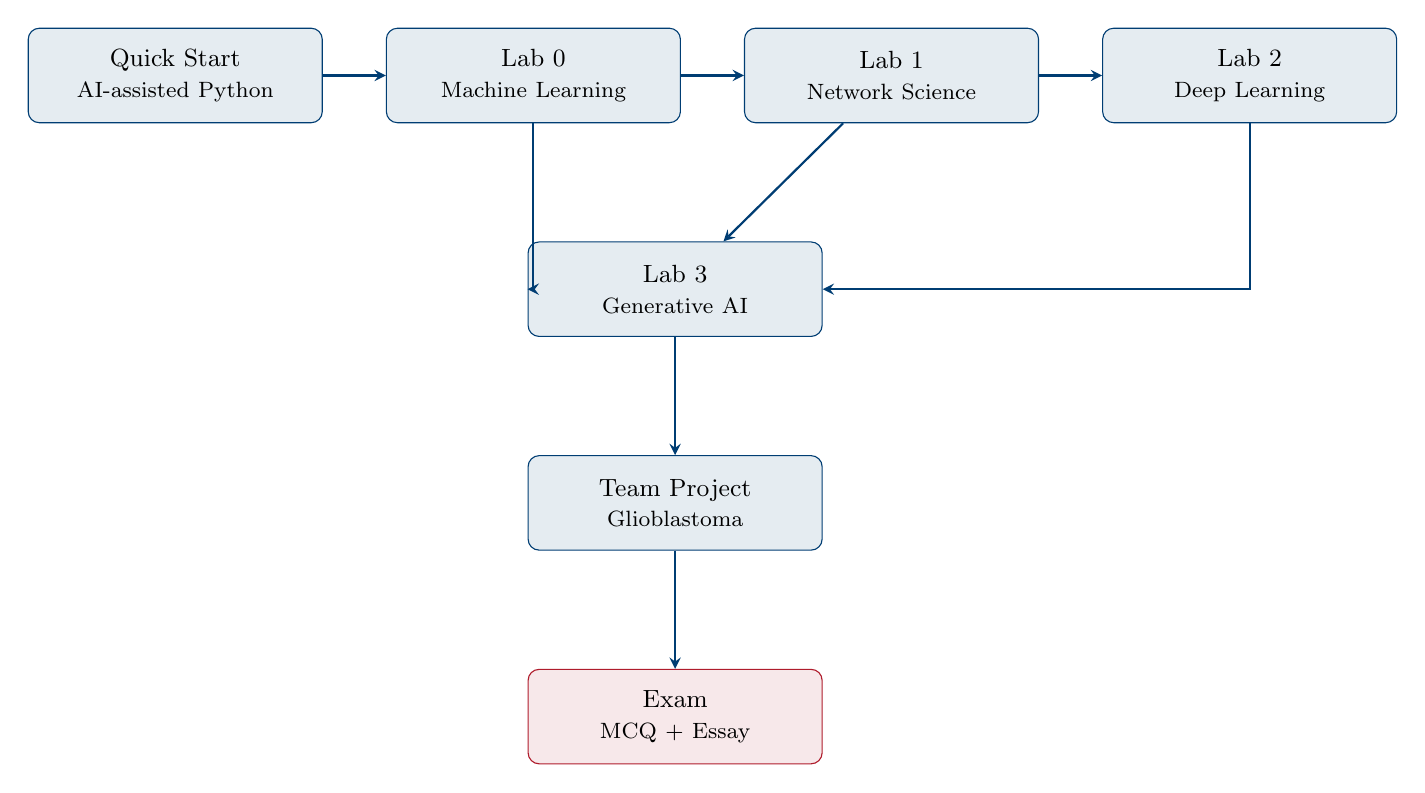
\begin{tikzpicture}[
    node distance=0.8cm,
    box/.style={rectangle, draw=uibblue, fill=uibblue!10, 
        text width=3.5cm, text centered, rounded corners, minimum height=1.2cm, font=\small},
    arrow/.style={thick,->,>=stealth,uibblue}
]
    % Row 1: Labs
    \node[box] (quickstart) {Quick Start\\{\footnotesize AI-assisted Python}};
    \node[box, right=of quickstart] (lab0) {Lab 0\\{\footnotesize Machine Learning}};
    \node[box, right=of lab0] (lab1) {Lab 1\\{\footnotesize Network Science}};
    \node[box, right=of lab1] (lab2) {Lab 2\\{\footnotesize Deep Learning}};
    
    % Row 2
    \node[box, below=1.5cm of lab0, xshift=1.8cm] (lab3) {Lab 3\\{\footnotesize Generative AI}};
    
    % Row 3
    \node[box, below=1.5cm of lab3] (team) {Team Project\\{\footnotesize Glioblastoma}};
    
    % Row 4
    \node[box, below=1.5cm of team, fill=uibred!10, draw=uibred] (exam) {Exam\\{\footnotesize MCQ + Essay}};
    
    % Arrows
    \draw[arrow] (quickstart) -- (lab0);
    \draw[arrow] (lab0) -- (lab1);
    \draw[arrow] (lab1) -- (lab2);
    \draw[arrow] (lab0) |- (lab3);
    \draw[arrow] (lab1) -- (lab3);
    \draw[arrow] (lab2) |- (lab3);
    \draw[arrow] (lab3) -- (team);
    \draw[arrow] (team) -- (exam);
\end{tikzpicture}
\caption{Course structure and progression in BMED365}
\label{fig:coursestructure}
\end{figure}

\subsection{AI in Medicine -- Main Topics}

\begin{figure}[htbp]
\centering
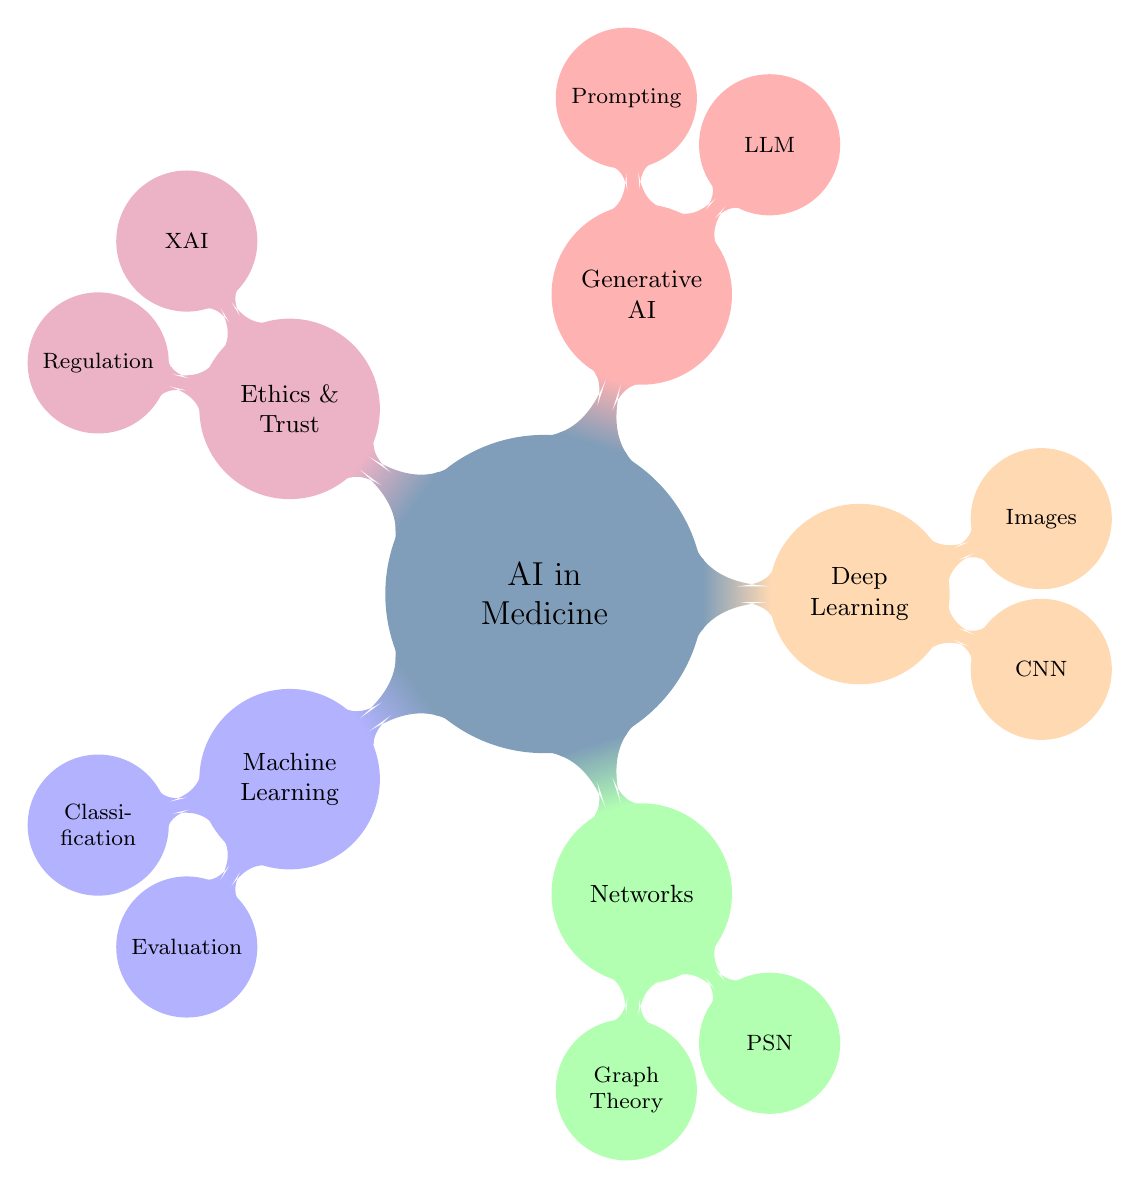
\begin{tikzpicture}[
    mindmap,
    grow cyclic,
    every node/.style={concept, execute at begin node=\hskip0pt},
    concept color=uibblue!50,
    level 1/.append style={level distance=4cm, sibling angle=72},
    level 2/.append style={level distance=2.5cm, sibling angle=45}
]
    \node[concept] {AI in\\Medicine}
        child [concept color=blue!30] { node {Machine\\Learning}
            child { node {Classification} }
            child { node {Evaluation} }
        }
        child [concept color=green!30] { node {Networks}
            child { node {Graph Theory} }
            child { node {PSN} }
        }
        child [concept color=orange!30] { node {Deep\\Learning}
            child { node {CNN} }
            child { node {Images} }
        }
        child [concept color=red!30] { node {Generative\\AI}
            child { node {LLM} }
            child { node {Prompting} }
        }
        child [concept color=purple!30] { node {Ethics \&\\Trust}
            child { node {XAI} }
            child { node {Regulation} }
        };
\end{tikzpicture}
\caption{Main topics in BMED365: Computational Imaging, Modeling and AI in Biomedicine}
\label{fig:topics}
\end{figure}

\end{document}
